\documentclass[12pt]{article}

\usepackage{amsmath}
\usepackage{epsfig}
\usepackage{varioref}

\title{A Mathematical Object System}
\author{Luke Palmer}

\begin{document}

\maketitle

\tableofcontents

\section{Problems}
\label{problems}
\subsection{Circle/Ellipse}

A classic example of a difficult theoretical problem is the
Circle/Ellipse problem.  Should Circle be derived from Ellipse?  A
Circle behaves like an Ellipse with identical foci, so isn't it a type
of Ellipse?  Or conversely, an Ellipse is a Circle with ``extended''
functionality, so isn't Ellipse derived from Circle?

Circle can't be derived from Ellipse, because you could pass your Circle
to a procedure as an Ellipse, then that procedure could try to change
one of the foci.  Alternatively, an Ellipse can't be derived from
Circle, since you can't find the radius of an Ellipse.

The conventional solution, then, is to make them siblings in your
heirarchy (if you still think the ``class heirarchy'' is a good way to
design your objects).  Indeed they are both shapes.  But it goes against
intuition that \textit{all circles are ellipses}.  This type of problem
has caught many object-oriented programmers off guard.

\subsection{Scalar Polymorphism}

A closely related problem arises in Perl's types.  A string can be used
as a number if it looks like a number, and any number can be used as a
string.  They ``convert'' to each other.  What is the inheritance
relationship between these two things?  They have, not similar, but
\textit{identical} usage properties; each can be used as the other.  We
say they are \textbf{automorphic}.

And yet, they must be siblings in the heirarchy for the same reason as
the Circle/Ellipse problem.  A number might be changed by the string
interface deeming it no longer a number.  A string isn't a type of
number because not all strings can be substituted for numbers.  We have
the same problem, and it's very hard to think about.

\subsection{Multimethods}

\label{problem:multimethods}

This is the most important refactorization that the paper introduces, so
I'll take some time to identify the problem.  I'll use a practical
example, one of the most common uses of multimethods: collision response
in a game.

Let's say you're making an Asteroids game.  You have a class heirarchy
as shown in figure \vref{mmd_prerefactor}.  In order to determine what
happens when two things collide, you've defined a multimethod
$\mathit{collide}$ with \textbf{manhattan distance} semantics.  It is
not defined symmetrically, because you preorder the arguments based on
which thing is moving faster (don't ask why).

\begin{figure}
\epsfig{file=MMD1.eps,width=4in}
\caption{Inheritance heirarchy of Asteroids game}
\label{mmd_prerefactor}
\end{figure}

\begin{figure}
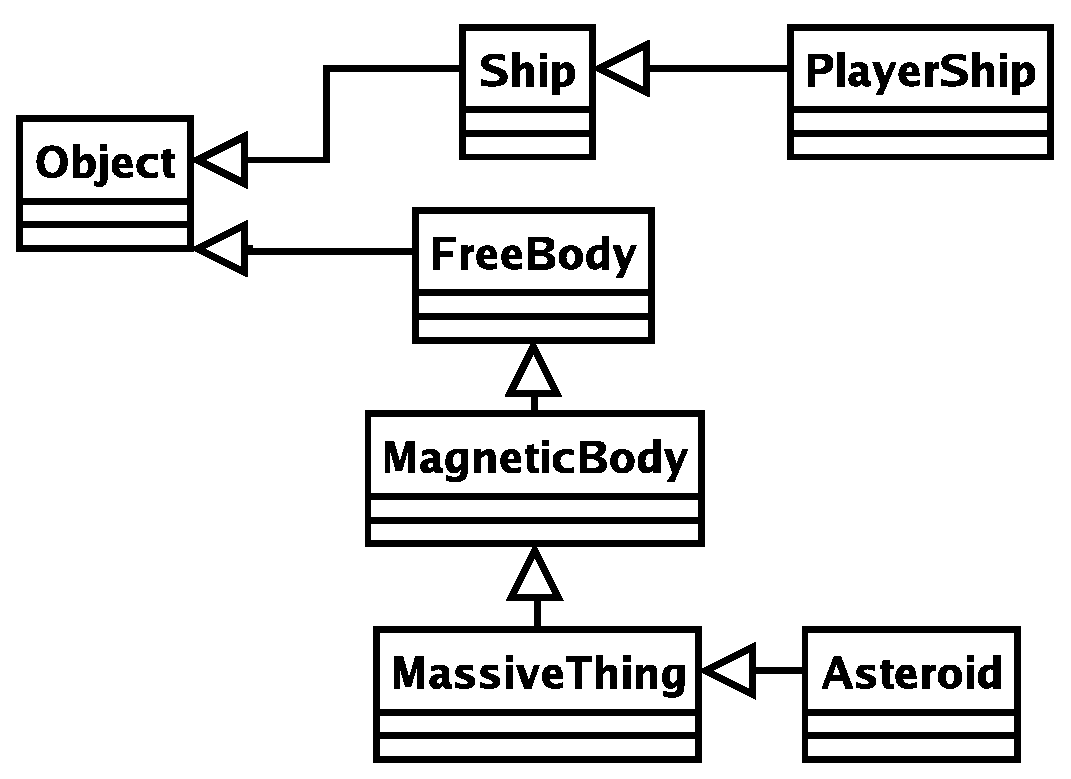
\epsfig{file=MMD2.eps,width=4in}
\caption{Inheritance heirarchy after refactoring}
\label{mmd_postrefactor}
\end{figure}

You have two implementations defined:
$\mathit{collide}_1(\mathit{MassiveThing}, \mathit{Object})$ and
$\mathit{collide}_2(\mathit{Object}, \mathit{PlayerShip})$.  During the
game, an $\mathit{Asteroid}$ collides with the $\mathit{PlayerShip}$.
The manhattan distance algorithm reasons as follows:

\begin{align*}
& d([\mathit{Asteroid},\mathit{PlayerShip}], \mathit{collide}_1) \\
& = \quad d(\mathit{Asteroid}, \mathit{MassiveThing}) + 
    d(\mathit{PlayerShip}, \mathit{Object}) \\
& = \quad 1 + 2 = 3 \\ 
& d([\mathit{Asteroid},\mathit{PlayerShip}], \mathit{collide}_2) \\
& = \quad d(\mathit{Asteroid}, \mathit{Object}) + 
    d(\mathit{PlayerShip}, \mathit{PlayerShip}) \\
& = \quad 2 + 0 = 2
\end{align*}

Thus, $\textit{collide}_2$ should be called, and the player
happily dies when he gets hit.

You decide that it's time for a refactor.  You want more in your game
than just asteroids.  So you add two classes above
$\textit{MassiveThing}$ and refactor some of $\textit{MassiveThing}$'s
code into them.  You end up with an inheritance heirarchy like figure
\vref{mmd_postrefactor}.  You didn't change anything, you just moved
some code around to make it easier to manage.

After the refactor, an $\mathit{Asteroid}$ collides with the
$\mathit{PlayerShip}$.  The manhattan distance algorithm reasons as
follows:

\begin{align*}
& d([\mathit{Asteroid},\mathit{PlayerShip}], \mathit{collide}_1) \\
& = \quad d(\mathit{Asteroid}, \mathit{MassiveThing}) + 
    d(\mathit{PlayerShip}, \mathit{Object}) \\
& = \quad 1 + 2 = 3 \\ 
& d([\mathit{Asteroid},\mathit{PlayerShip}], \mathit{collide}_2) \\
& = \quad d(\mathit{Asteroid}, \mathit{Object}) + 
    d(\mathit{PlayerShip}, \mathit{PlayerShip}) \\
& = \quad \mathbf{4} + 0 = \mathbf{4}
\end{align*}

Thus, $\mathit{collide}_1$ should be called, and the player flies off
into the distance like a piece of debris when hit by the asteroid, but
does not die.  The player is very disappointed\footnote{This seems to be
a morbid and suicidal player.}.

You can see how a simple refactor greatly changed which implementation
was chosen.  Imagine if someone wrote a module with a class, and someone
else wrote a module that defined interactions between that class and the
rest of the world.  These two modules become tightly coupled, and it's
impossible to change the class heirarchy in the former without modifying
the latter.  This is clearly against what one would call an
``object-oriented virtue.''

Programmers have an expectation when working with inheritance, and a
very valid one at that.  That is, ``If I derive a new class $B$ from a
class $A$ and don't put anything in the definition, it should work
exactly like $A$.''  Again, this is violated by manhattan distance.

\section{Theory}
\subsection{The Axiom}

The entire theory follows from one axiom: \textbf{All objects are
constant}.  Don't worry, the next section will address any fears you
have about this changing the procedural paradigm.  It all works out.

Taking this axiom, we are suddenly able to state inheritance and other
types of relationships in terms of mathematical sets.  We state several
definitions, mapping computer science jargon onto mathematical jargon:

\begin{itemize}
\item A \textbf{class} is the set of all instances of that class,
whether or not they have been instantiated yet.  Classes are also
objects, and they are members of the class \textit{Class}.

\item A \textbf{role} is the set of all objects that compose that role.

\item A \textbf{subclass} (implementation derivation with interface
compatibility) is a relationship of set containment.  If $A \,
\mathit{isa} \, B$ then $A \subseteq B$ ($A$ is an improper subset of
$B$).

\item A \textbf{subtype} (value restriction on a general type) is
\textit{also} a containment relationship.  If $A \, \mathit{restricts}
\, B$ then $A \subseteq B$.  Note that there is no mathematical
difference whatsoever between subclassing and subtyping.

\item A \textbf{procedure} is an object that can be invoked at a
particular point in time to manipulate the state of the program.  It may
``return'' a value, and that value may be different for the same
arguments upon different invocations.  The word \textbf{function} is
reserved for constant, side-effect-free relationships, though I'll use
the word \textbf{map} to avoid ambiguity.

\item A \textbf{method} is a map from an object to a procedure.  Calling
a method $M$ on an object $x$ involves calling the procedure that the
map returns: $\mathit{call}\,Mx$.

\end{itemize}

\subsection{References}

In order to keep the procedural paradigm, \textbf{references} must be
introduced.  They are \textit{not} objects, since they can be changed
over the course of execution.  A reference refers to an object or
another reference.

A \textbf{variable} (as defined by computer science) is just a named
reference.  References can also be \textbf{typed}, which means that they
can only ever refer to objects of a particular class or references
thereof.  If a reference is \textbf{untyped}, then it may refer to
anything at any point.

Objects with value semantics in oldspeak are just objects, whereas
objects with referential semantics are references.  Most such references
are typed references.

This is how it is possible to modify objects (if they have referential
semantics---you can't modify objects with value semantics).  Say you
have an object $A$ with a \textbf{member variable} $x$.  If you wish to
increment $x$, you map the object to a new one $B$ where $B.x = A.x +
1$, and then point the reference to $B$ instead of $A$.

Note that this operation sometimes changes the type.  Supposeyou have a
subtype $\mathit{int8}$ of $\mathit{int}$, where an $\mathit{int8}\,x
\in [0,256)$.  Then if the object's is 255, and you increment it (which,
as defined above, is performing the operation and remapping the
reference), then it is no longer an $\mathit{int8}$.  If the reference
was typed as $\mathit{int8}$, then you get a type error, but it is
perfectly valid for an untyped reference.

\subsection{Automorphism}

An \textbf{automorphism} is a map between two logically equivalent
objects that are implemented differently.  The ``auto'' is a bit of a
pun: it means both ``self'' and ``automatic''.  

Using automorphisms you can define a subset relationship without using
implementation derivation or subtyping.  This is often necessary.  For
example, take a $\mathit{Real}$ class and a $\mathit{Complex}$ class.
One would hardly want to define $\mathit{Real}$ as a subtype of
$\mathit{Complex}$, since it's a waste of time and memory.  However, all
$\mathit{Real}$s are $\mathit{Complex}$es, so you'd want to state that
this relationship holds.  You would define an automorphism from
$\mathit{Real}$ to $\mathit{Complex}$, so that $\mathit{Real}$s can be
used as $\mathit{Complex}$es without being implemented by them.

On the practical side, this also allows you to create a superclass
\textit{a posteriori}.  The $\mathit{Complex}$ / $\mathit{Real}$ example
comes to mind again, $\mathit{Real}$ being a ``built-in'' type and
$\mathit{Complex}$ a user-defined type.

\subsection{Multimethods}

In defining multimethods in a mathematically rigorous way, we would like
to avoid the problems from section \ref{problem:multimethods}.  If we
look hard enough, we can see the logical flaw in manhattan distance's
reasoning.  It is a flaw that won't be solved by cartesian or any other
sort of distance.  It is the practice of measuring the distance in the
first place that is the flaw.

\begin{figure}
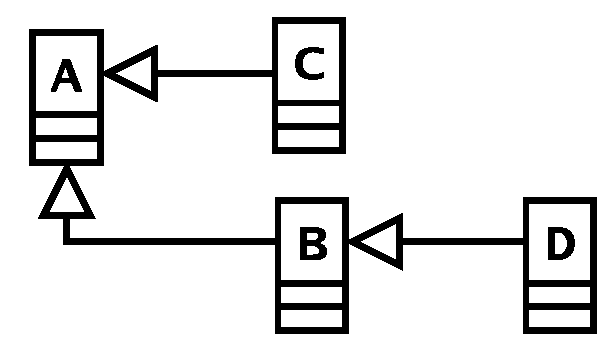
\epsfig{file=MMD3.eps,width=3in}
\caption{A class heirarchy}
\label{mmd_example}
\end{figure}

Consider four classes $A$, $B$, $C$, and $D$ where $B \subseteq A$, $C
\subseteq A$, and $D \subseteq B$, depicted in figure \vref{mmd_example}.
When measuring distances in multimethod dispatch, they say that $D$ is
\textit{more derived} than $B$ (from $A$).  This is understandable,
since $D \subseteq B$.  It is also said that $D$ is \textit{more
derived} than $C$, since there are more classes between it and $A$.  To
make matters worse, it is said that $D$ is \textit{exactly twice as
derived} as $C$.

Let's ponder this:  Is it possible that $D$ have 50 elements and $C$
have only one?  Sure.  Is it even possible that $C \subseteq D$?  Yes.
So how can $D$ be more derived than $C$?  We have found the flaw.  This
definition has no foundation in logic: it is just an arbitrary choice.
``How many classes separate the two?''  What does that have to do with
\textit{anything}?

Fortunately, our new system leads us away from that travesty.  In
particular, the question ``how many classes separate the two'' can't
even be asked, since a class is a set, and one can ponder infinitely
many sets between any two classes in the general case.  All we have to
work with are the relations between the sets.

Now we'll define the multimethod map $M$.  Let $\phi$ and $\psi$ be
procedures, and let $\alpha$ be the argument list.  $\phi_i$ refers to
the $i$th parameter type to $\phi$.  $\alpha_i$ refers to the actual
$i$th argument (not it's type!).  Then $M(\alpha)$ maps to $\phi$ only
if the following conditions hold:

\begin{enumerate}
\item For every valid $i$, $\alpha_i \in \phi_i$.
\item For every procedure $\psi \not= \phi$ for which (1) holds, $\phi_i
\subseteq \psi_i$ for every valid $i$ \textit{and} there is at least one
$j$ where $\psi_j \not\subseteq \phi_j$.
\end{enumerate}
 
If there is no such $\phi$ defined, then the dispatch is an error.

In layman's terms, rule (1) simply means that the arguments must match
the parameters.  Rule (2) means that if a method is to be picked, it
must be \textit{more specific} than any other matching method.
\textit{More specific} is defined such that an argument matching the
candidate's parameter implies matching the other's parameter, and there
is at least one parameter for which the reverse doesn't hold.

\section{Application}

In this section we'll see how this theory addresses the problems
described in section \ref{problems}.

\subsection{Circle/Ellipse}

Since all objects are constant, there is nothing stopping the intuitive
relation from holding, that Circle is a subclass Ellipse.  Or rather
that $\mathit{Circle} \subseteq \mathit{Ellipse}$, since there could be
an automorphism defined between Circle and Ellipse without actually
being implementation derived.

\subsection{Scalar Polymorphism}

This is another easy one.  Strings that look like numbers simply
\textit{are} numbers: they're the same exact objects.  Conversely, all
numbers are strings.  Then the relation is simple: $\mathit{Num}
\subseteq \mathit{Str}$.

\subsection{Multimethods}

The final section of the paper, the multimethod section, is again the
interesting one.  While the multimethod dispatch algorithm proposed in
this paper is certainly more logically sound than manhattan's, it isn't
without some worries.

In particular, note that this algorithm gives rise to ambiguity much
more often than manhattan---and there was too much ambiguity there
already.  The problem is alleviated through the introduction of
automorphism, requiring the programmer to rethink his relations rather
than twisting himself up in hundreds of very specific multimethod
definitions. 

Using the \textit{Real} and \textit{Complex} example that I mentioned
earlier, I'll give only a glimse of the beauty of the automorphism
technique.

Let's say we've written a \textit{Complex} class, with a $+$ multimethod
defined between pairs of \textit{Complex}es.  To get this to work with
\textit{Real}s, we define an automorphism from \textit{Real} to
\textit{Complex}, saying that any real number can be used as a complex
number.  It's obvious that this works:  any \textit{Real} is morphed
into a \textit{Complex}, and then the operations are carried out.

Now what happens if you define a modifying operation $+=$.  The left
side is a read-write argument; an argument with referential semantics.
It is still only defined between \textit{Complex} and \textit{Complex}.
This method can't be called, because there needs to be an automorphism
\textit{both ways} for a read-write argument to be passed.

In actuality, the language has a choice here.  What if the right hand
side were $4 + 0i$.  

\end{document}
